\documentclass{article}
\usepackage[UTF8]{ctex}
\usepackage[T1]{fontenc}
\usepackage[utf8]{inputenc}
\usepackage{float}
\usepackage{placeins}
\usepackage{latexsym}
\usepackage{amsmath}
\usepackage{amsthm}
\usepackage{amssymb}
\usepackage{listings}
\usepackage{xcolor}
\usepackage{ulem}
\usepackage{multicol}
\usepackage{geometry}
\usepackage{hyperref}
\usepackage{tikz}
\usetikzlibrary{positioning}
\usetikzlibrary[arrows, shapes, chains]
\hypersetup{
	colorlinks=true,
	urlcolor=black,
}
\lstset
{
    basicstyle = \ttfamily,
    keywordstyle = \bfseries\color{blue!70},
    commentstyle = \songti \upshape,
    escapeinside=``,
    breaklines = true,
    breakatwhitespace = true,
    breakautoindent = true,
    texcl = true,
    showstringspaces = false,
    basewidth = 0.5em,
    flexiblecolumns,
    columns = fixed,
    frame = {},
}
\lstdefinestyle{C}
{
    language = C,
}
\lstdefinestyle{Assembler}
{
    language = [X86masm]Assembler,
    alsolanguage = C,
}

\title{Homework 11}
\author{PB17000297 罗晏宸}
\date{November 13 2019}


\begin{document}

\maketitle

\section*{Exercise 1}
针对\href{http://staff.ustc.edu.cn/~qlzheng/compiler/lec10_2.ppt}{第十二讲 代码优化(2)}P31上流图,计算到达-定值数据流方程,并给出相应的ud链。

\begin{figure}[H]
    \centering
    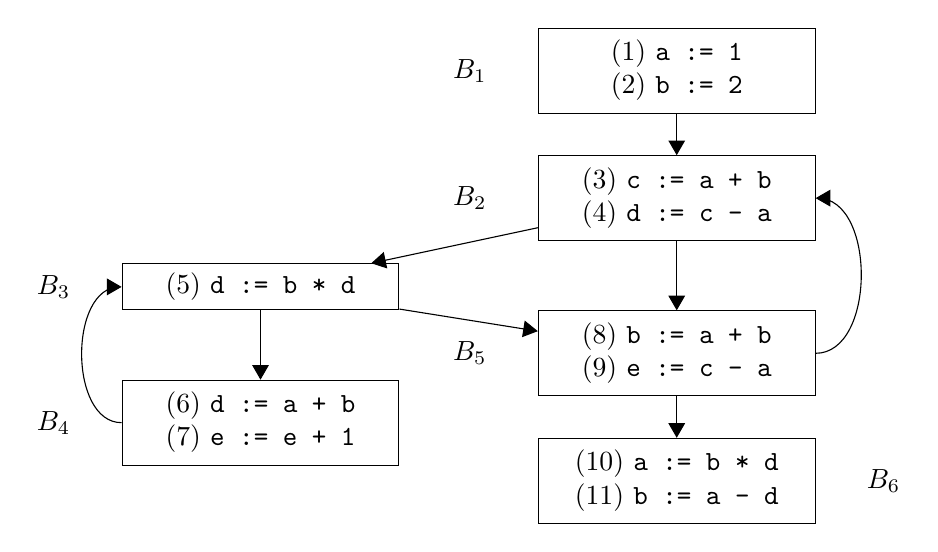
\begin{tikzpicture}[node distance = 1.5em]
        \tikzstyle{block} = [rectangle, draw=black, text ragged, minimum height = 1.6em, minimum width = 10em];
        \node [block]  (B1)
        {
            \begin{tabular}{l}
                (1) \texttt{a := 1} \\
                (2) \texttt{b := 2}
            \end{tabular}
        };
        \node [block, below = of B1]  (B2)
        {
            \begin{tabular}{l}
                (3) \texttt{c := a + b} \\
                (4) \texttt{d := c - a}
            \end{tabular}
        };
        \node [block, below left = 0.8em and 5.0em of B2]  (B3)  {(5) \texttt{d := b * d}};
        \node [block, below = 2.5em of B3]  (B4)
        {
            \begin{tabular}{l}
                (6) \texttt{d := a + b} \\
                (7) \texttt{e := e + 1}
            \end{tabular}
        };
        \node [block, below = 2.5em of B2]  (B5)
        {
            \begin{tabular}{l}
                (8) \texttt{b := a + b} \\
                (9) \texttt{e := c - a}
            \end{tabular}
        };
        \node [block, below = of B5]  (B6)
        {
            \begin{tabular}{l}
                (10) \texttt{a := b * d} \\
                (11) \texttt{b := a - d}
            \end{tabular}
        };
        \foreach \i in {1, ..., 5}
            \node [left = of B\i] (A\i) {$B_{\i}$};
        \node [right = of B6] (A6) {$B_{6}$};

        \foreach \i/\j in {1/2, 2/3, 2/5, 3/4, 3/5, 5/6}
            \draw [-triangle 60] (B\i) to [] (B\j);

        \draw [-triangle 60] (B4) to [out = 180, in = 180] (B3);
        \draw [-triangle 60] (B5) to [out = 0, in = 0] (B2);

    \end{tikzpicture}
    \caption{第十二讲 代码优化(2)P31上流图}
\end{figure}

\paragraph{解}
首先给出每个基本块的$gen$和$kill$集合
\begin{table}[H]
    \centering
    \begin{tabular}{|c|c|c|}
    \hline
    基本块 & $gen$ & $kill$ \\ \hline
    $B_1$ & $gen_1 = \{1,2\}$ & $kill_1 = \{8,10,11\}$ \\ \hline
    $B_2$ & $gen_2 = \{3,4\}$ & $kill_2 = \{5,6\}$ \\ \hline
    $B_3$ & $gen_3 = \{5\}$ & $kill_3 = \{4,6\}$ \\ \hline
    $B_4$ & $gen_4 = \{6,7\}$ & $kill_4 = \{4,5,9\}$ \\ \hline
    $B_5$ & $gen_5 = \{8,9\}$ & $kill_5 = \{2,7,11\}$ \\ \hline
    $B_6$ & $gen_6 = \{10,11\}$ & $kill_6 = \{1,2,8\}$ \\ \hline
    \end{tabular}
\end{table}
初始值
\begin{align*}
   & \text{IN}[B_1] = \text{IN}[B_2] = \text{IN}[B_3] = \text{IN}[B_4] = \text{IN}[B_5] = \text{IN}[B_6] = \varnothing \\
   & \text{OUT}[B_1] = gen_1 = \{1,2\} \\
   & \text{OUT}[B_2] = gen_2 = \{3,4\} \\
   & \text{OUT}[B_3] = gen_3 = \{5\} \\
   & \text{OUT}[B_4] = gen_4 = \{6,7\} \\
   & \text{OUT}[B_5] = gen_5 = \{8,9\} \\
   & \text{OUT}[B_6] = gen_6 = \{10,11\}
\end{align*}
第一次迭代
\begin{align*}
   & \text{IN}[B_1] = \varnothing &&&&&\\
   & \text{OUT}[B_1] &&= gen_1 \cup (\text{IN}[B_1] - kill_1) &&= gen_1 &= \{1,2\} \\
   & \text{IN}[B_2] &&= \text{OUT}[B_1] \cup \text{OUT}[B_5] &&&= \{1,2,8,9\}\\
   & \text{OUT}[B_2] &&= gen_2 \cup (\text{IN}[B_2] - kill_2) &&= \{3,4\} \cup \{1,2,8,9\} &= \{1,2,3,4,8,9\} \\
   & \text{IN}[B_3] &&= \text{OUT}[B_2] \cup \text{OUT}[B_4] &&&= \{1,2,3,4,6,7,8,9\}\\
   & \text{OUT}[B_3] &&= gen_3 \cup (\text{IN}[B_3] - kill_3) &&= \{5\} \cup \{1,2,3,7,8,9\} &= \{1,2,3,5,7,8,9\} \\
   & \text{IN}[B_4] &&= \text{OUT}[B_3] &&&= \{1,2,3,5,7,8,9\}\\
   & \text{OUT}[B_4] &&= gen_4 \cup (\text{IN}[B_4] - kill_4) &&= \{6,7\} \cup \{1,2,3,7,8\} &= \{1,2,3,6,7,8\} \\
   & \text{IN}[B_5] &&= \text{OUT}[B_2] \cup \text{OUT}[B_3] &&&= \{1,2,3,4,5,7,8,9\}\\
   & \text{OUT}[B_5] &&= gen_5 \cup (\text{IN}[B_5] - kill_5) &&= \{8,9\} \cup \{1,3,4,5,8,9\} &= \{1,3,4,5,8,9\} \\
   & \text{IN}[B_6] &&= \text{OUT}[B_5] &&&= \{1,3,4,5,8,9\}\\
   & \text{OUT}[B_6] &&= gen_6 \cup (\text{IN}[B_6] - kill_6) &&= \{10,11\} \cup \{3,4,5,9\} &= \{3,4,5,9,10,11\}
\end{align*}
第二次迭代
\begin{align*}
    & \text{IN}[B_1] = \varnothing &&&&&\\
    & \text{OUT}[B_1] &&= gen_1 \cup (\text{IN}[B_1] - kill_1) &&= gen_1 &= \{1,2\} \\
    & \text{IN}[B_2] &&= \text{OUT}[B_1] \cup \text{OUT}[B_5] &&&= \{1,2,3,4,5,8,9\} \\
    & \text{OUT}[B_2] &&= gen_2 \cup (\text{IN}[B_2] - kill_2) &&= \{3,4\} \cup \{1,2,3,4,8,9\} &= \{1,2,3,4,8,9\} \\
    & \text{IN}[B_3] &&= \text{OUT}[B_2] \cup \text{OUT}[B_4] &&&= \{1,2,3,4,6,7,8,9\} \\
    & \text{OUT}[B_3] &&= gen_3 \cup (\text{IN}[B_3] - kill_3) &&= \{5\} \cup \{1,2,3,7,8,9\} &= \{1,2,3,5,7,8,9\} \\
    & \text{IN}[B_4] &&= \text{OUT}[B_3] &&&= \{1,2,3,5,7,8,9\} \\
    & \text{OUT}[B_4] &&= gen_4 \cup (\text{IN}[B_4] - kill_4) &&= \{6,7\} \cup \{1,2,3,7,8\} &= \{1,2,3,6,7,8\} \\
    & \text{IN}[B_5] &&= \text{OUT}[B_2] \cup \text{OUT}[B_3] &&&= \{1,2,3,4,5,7,8,9\} \\
    & \text{OUT}[B_5] &&= gen_5 \cup (\text{IN}[B_5] - kill_5) &&= \{8,9\} \cup \{1,3,4,5,8,9\} &= \{1,3,4,5,8,9\} \\
    & \text{IN}[B_6] &&= \text{OUT}[B_5] &&&= \{1,3,4,5,8,9\} \\
    & \text{OUT}[B_6] &&= gen_6 \cup (\text{IN}[B_6] - kill_6) &&= \{10,11\} \cup \{3,4,5,9\} &= \{3,4,5,9,10,11\}
\end{align*}
迭代终止。ud链如下
\begin{itemize}
    \item (3)(4)(6)(8)(9)中\texttt{a}的引用的ud链为(1)\texttt{a := 1};(11)中\texttt{a}的引用的ud链为(10)\texttt{a := b * d}
    \item (3)(5)(6)(8)中\texttt{b}的引用的ud链为(2)\texttt{b := 2},(10)中\texttt{b}的引用的ud链为(8)\texttt{b := a + b}
    \item (4)(9)中\texttt{c}引用的ud链为(3)\texttt{c := a + b}
    \item (5)中\texttt{d}引用的ud链为(6)\texttt{d := a + b }(4)\texttt{d := c - a};(6)中\texttt{d}引用的ud链为(5)\texttt{d := b * d};(10)(11)中\texttt{d}引用的ud链为(4)\texttt{d := c - a }(5)\texttt{d := b * d}
    \item (7)中\texttt{e}引用的ud链为(7)\texttt{e := e + 1 }(9)\texttt{e := c - a}
\end{itemize}

\section*{Exercise 2}
针对以下C函数,给出其函数体三地址码,流图及自然循环。

\begin{lstlisting}[style = C]
#define N 32

int a[N], b[N];
int arr[N + 1][N + 1];

void lcs()
{
    for (i = 1; i <= length1; ++i)
    {
        for (j = 1; j <= length2; ++j)
        {
            if (a[i - 1] == b[j - 1]) // 串中的下标从0开始
            {
                arr[i][j] = arr[i - 1][j - 1] + 1;
            }
            else
            {
                arr[i][j] = arr[i - 1][j] > arr[i][j - 1] ? arr[i - 1][j] : arr[i][j - 1];
            }
        }
    }
}
\end{lstlisting}

\paragraph{解}
首先给出三地址中间代码结构
\begin{lstlisting}[language = Pascal, alsolanguage = C, lineskip = 0.1em]
    i = 1
L1: t1 = a - 128
    t2 = b - 128
L2: j = 1
    t3 = i - 1
    t4 = j - 1
    t5 = t1[t3]
    t6 = t2[t4]
    t8 = arr - 132
    t7 = i * 33
    t7 = t7 + j
    t7 = t7 * 4
    if t5 != t6 goto L3
    t9 = t3 * 33
    t9 = t9 + t4
    t9 = t9 * 4
    t10 = t8[t9]
    t10 = t10 + 1
    t8[t7] = t10
    goto L5
L3: t11 = i - 1
    t11 = t11 * 33
    t11 = t11 + j
    t11 = t11 * 4
    t12 = i * 33
    t12 = t12 + j
    t12 = t12 - 1
    t12 = t12 * 4
    t13 = t8[t11]
    t14 = t8[t12]
    if t13 <= t14 goto L4
L4: t8[t7] = t11
    goto L5
    t8[t7] = t12
L5: j = j + 1
    if j <= length2 goto L2
    i = i + 1
    if i <= length1 goto L1
    \end{lstlisting}

据此构建流图,并列出自然循环:
\begin{itemize}
    \item 回边$B_8 \rightarrow B_3$:循环$B_3, B_4, B_5, B_6, B_7, B_8$
    \item 回边$B_9 \rightarrow B_2$:循环$B_2, B_3, B_4, B_5, B_6, B_7, B_8, B_9$
\end{itemize}

\newgeometry{left = 0em, right = 0em}
\begin{figure}
    \centering
    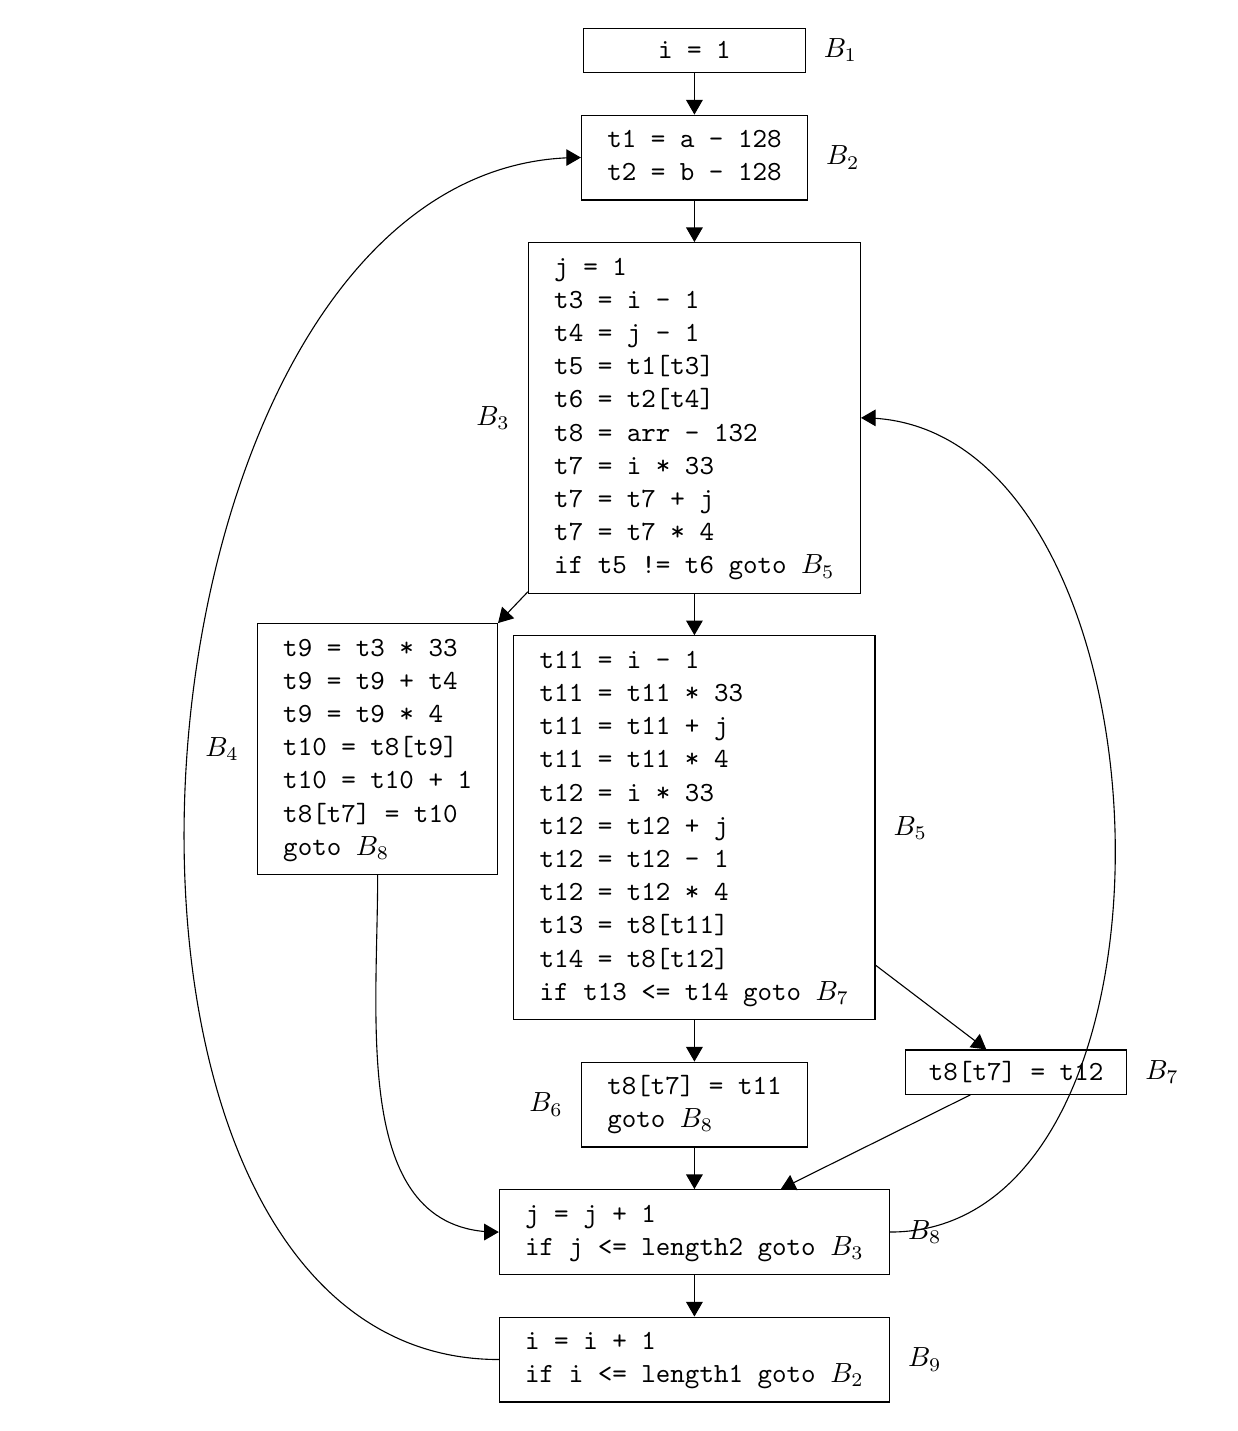
\begin{tikzpicture}[node distance = 1.5em]
        \tikzstyle{block} = [rectangle, draw=black, text ragged, minimum height = 1.6em, minimum width = 8em];
        \node [block]                       (B1) {\texttt{i = 1}};
        \node [block, below = of B1]        (B2)
        {
            \begin{tabular}{l}
                \texttt{t1 = a - 128} \\
                \texttt{t2 = b - 128}
            \end{tabular}
        };
        \node [block, below = of B2]        (B3)
        {
            \begin{tabular}{l}
                \texttt{j = 1} \\
                \texttt{t3 = i - 1} \\
                \texttt{t4 = j - 1} \\
                \texttt{t5 = t1[t3]} \\
                \texttt{t6 = t2[t4]} \\
                \texttt{t8 = arr - 132} \\
                \texttt{t7 = i * 33} \\
                \texttt{t7 = t7 + j} \\
                \texttt{t7 = t7 * 4} \\
                \texttt{if t5 != t6 goto }$B_{5}$
            \end{tabular}
        };
        \node [block, below left = of B3]   (B4)
        {
            \begin{tabular}{l}
                \texttt{t9 = t3 * 33} \\
                \texttt{t9 = t9 + t4} \\
                \texttt{t9 = t9 * 4} \\
                \texttt{t10 = t8[t9]} \\
                \texttt{t10 = t10 + 1} \\
                \texttt{t8[t7] = t10} \\
                \texttt{goto }$B_{8}$
            \end{tabular}
        };
        \node [block, below = of B3]  (B5)
        {
            \begin{tabular}{l}
                \texttt{t11 = i - 1} \\
                \texttt{t11 = t11 * 33} \\
                \texttt{t11 = t11 + j} \\
                \texttt{t11 = t11 * 4} \\
                \texttt{t12 = i * 33} \\
                \texttt{t12 = t12 + j} \\
                \texttt{t12 = t12 - 1} \\
                \texttt{t12 = t12 * 4} \\
                \texttt{t13 = t8[t11]} \\
                \texttt{t14 = t8[t12]} \\
                \texttt{if t13 <= t14 goto }$B_{7}$
            \end{tabular}
        };
        \node [block, below = of B5]   (B6)
        {
            \begin{tabular}{l}
                \texttt{t8[t7] = t11} \\
                \texttt{goto }$B_{8}$
            \end{tabular}
        };
        \node [block, below right = of B5]  (B7)  {\texttt{t8[t7] = t12}};
        \node [block, below = of B6]  (B8)
        {
            \begin{tabular}{l}
                \texttt{j = j + 1} \\
                \texttt{if j <= length2 goto }$B_{3}$
            \end{tabular}
        };
        \node [block, below = of B8]  (B9)
        {
            \begin{tabular}{l}
                \texttt{i = i + 1} \\
                \texttt{if i <= length1 goto }$B_{2}$
            \end{tabular}
        };


        \foreach \i in {1, 2, 5, 7, 8, 9}
            \node [right = 0.3em of B\i] (A\i) {$B_{\i}$};
        \foreach \i in {3, 4, 6}
            \node [left = 0.3em of B\i] (A\i) {$B_{\i}$};

        \foreach \i/\j in {1/2, 2/3, 3/4, 3/5, 5/6, 5/7, 6/8, 7/8, 8/9}
            \draw [-triangle 60] (B\i) to [] (B\j);

        \draw [-triangle 60] (B4) to [out = -90, in = 180] (B8);
        \draw [-triangle 60] (B8) to [out = 0, in = 0] (B3);
        \draw [-triangle 60] (B9) to [out = 180, in = 180] (B2);
    \end{tikzpicture}
    \caption{C代码对应流图}
\end{figure}
\restoregeometry

\end{document}

